\section{System Architecture}
\label{sec:system-architecture}
We start our system architecture design from several key application requirements, mainly the users' point of view.

Imagine one wants to know his indoor location without painful process of looking at room number and comparing it with a sophiscated map; the system should be able to detect his location and automatically generate the highlighted location with the display of a map. Meanwhile, {\bf privacy} is an important issue that the localization should be computed locally and the user is able to control whether to share his location or not. Good {\bf accuracy} and {\bf responsiveness} are also required to ensure users' satisfaction of this system.  

In addition to the local display of location, interesting applications can be built upon the aggregation of users' information. We design one such application called Marauder's Map\footnote{http://en.wikipedia.org/wiki/Magical\_objects\_in\_Harry\_Potter\#The\_Marauder.27s\_Map}, which could show the active location of other users. This requires the front-end and back-end design to provide {\bf accessibility} of the aggregated information. Also since location is changing rapidly and would only be meaningful within a short amount of time, real-time communication ({\bf timeliness}) is often desired.

\begin{figure}
  \centering
  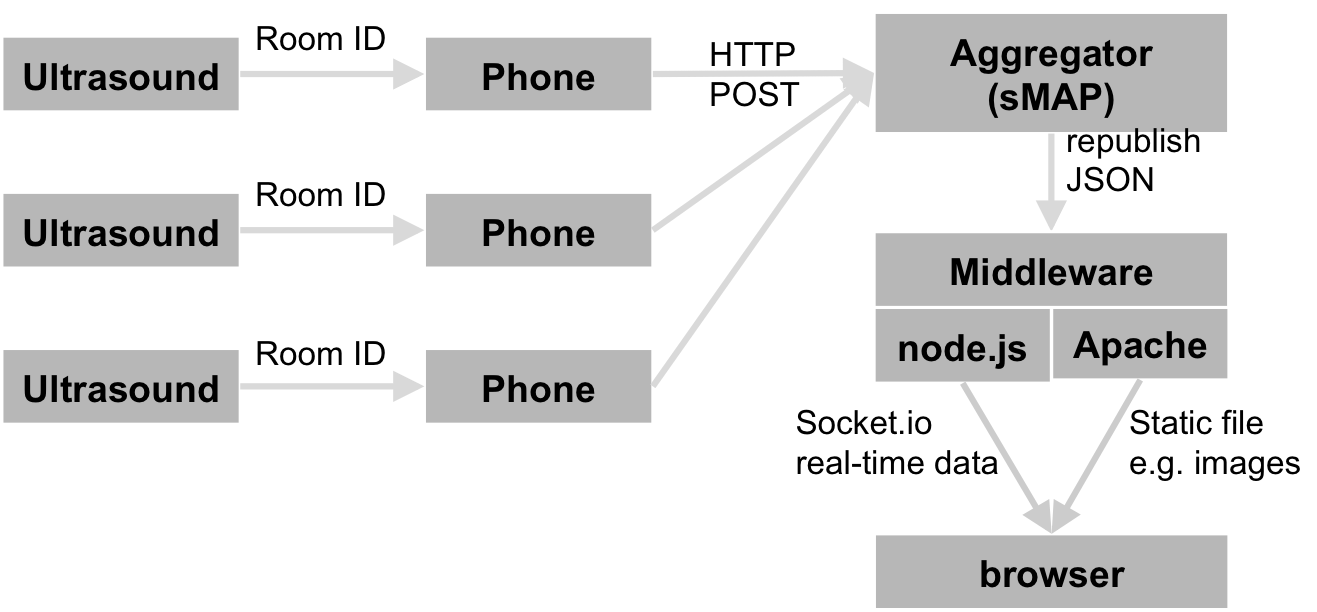
\includegraphics[width=\columnwidth]{sysarch.png}
  \caption{System Architecture for Marauder's Map}
  \label{fig:sysarch}
\end{figure}

Our system architecture is shown in Fig.\,\ref{fig:sysarch} where each room will be installed with an ultrasound beacon to broadcast room ID. Smartphones act as receivers to process the audio recording and decode this ID. The signal design and filtering algorithm are fully covered in Sec.\,\ref{sec:android-application}, which mainly address the requirement of {\bf accuracy} and {\bf responsiveness}. The user can use stand-alone map to view his live location, or config the entire system to publish his location to the back end server through HTTP POST ({\bf privacy}). Such aggregation of multiple users' location is now achieved by sMAP~\cite{dawson2010smap} server, which supports republishing to any subscribers {\bf accessibility}. There is a middleware we implemented to interface between any client (potentially browsers) and the sMAP server. Such middleware not only provides front-end user interface (HTML webpage, CSS, static images, javascript), but also act as subscribers of sMAP to enable real-time communication {\bf timeliness} to browsers, through Socket.IO~\cite{socketio} technology. Next section will be the details of our project implementation of each functional block in the system.

%% Master
%%% Local Variables: 
%%% mode: latex
%%% TeX-master: "ee149"
%%% End: 
